\documentclass{article}
\usepackage[utf8]{inputenc}
\usepackage{hyperref}
\usepackage{graphicx}
\usepackage{float}
\usepackage{enumitem}

\title{PigeonHole UGent Submission Platform User Manual}
\author{SEL group 1 2024}
\date{\today}

\begin{document}

\maketitle

\tableofcontents

\section{Introduction}
Welcome to the PigeonHole UGent Submission Platform User Manual. This manual provides instructions for users, teachers, and administrators on how to effectively use the platform, step by step. The platform is designed to streamline the process of submitting, reviewing, and providing feedback on projects. It seeks to create a middle ground between being easy to use but also providing the necessary features for automatic feedback on big projects. As for now, we only support UGent accounts to use the platform.

\section{Getting Started}
\subsection{Creating an Account}
Users can only log in with their UGent account. If you do not have an account, please contact the administrator to create one for you.

\subsection{Logging In}
When accessing the platform, students will be prompted to log in with their UGent account. UGent uses OAuth2 for authentication, so you will be redirected to the UGent login page. After logging in, you will be redirected back to the platform.

\begin{figure}[H]
    \centering
    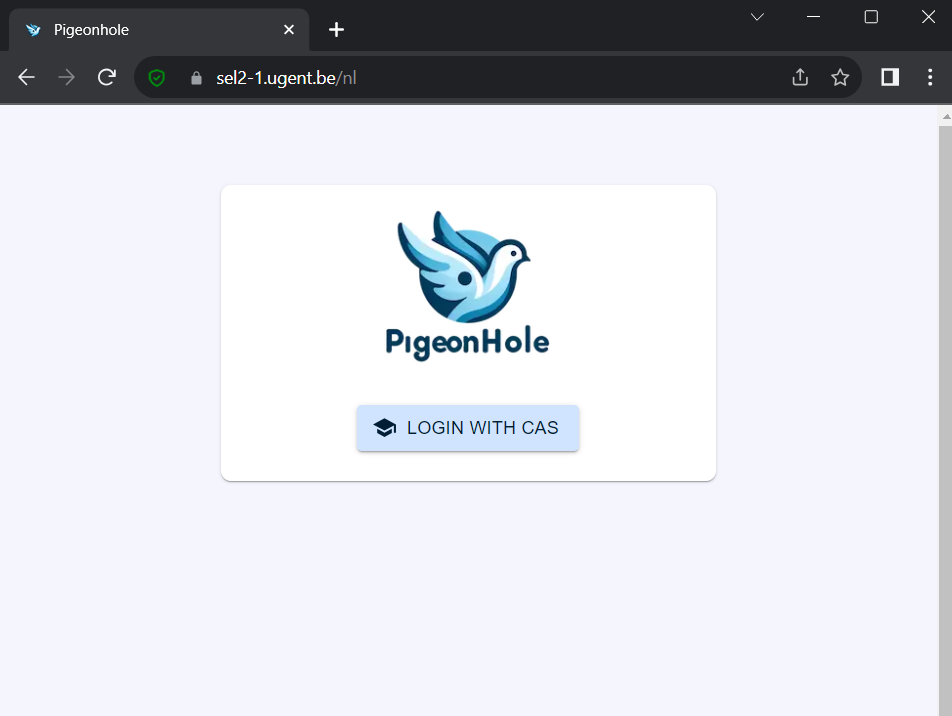
\includegraphics[width=0.75\textwidth]{images/login.png}
    \caption{Login Screen}
\end{figure}

\subsection{Changing language}
We support English and Dutch. You can change in the small dropdown menu in the top right corner of every page's topbar.

\subsection{Changing your profile picture}
By clicking on your name in the top right corner of the page, you can navigate to your profile page. Here you can change your profile picture by clicking on the image, selecting a new image, and clicking save.

\section{Student Section}

\subsection{View your courses}

You can view all courses you are enrolled in and the projects that are available for submission central on the homepage. By clicking on a course title you can navigate to the course page, by clicking view project you can navigate to the project page.

\begin{figure}[H]
    \centering
    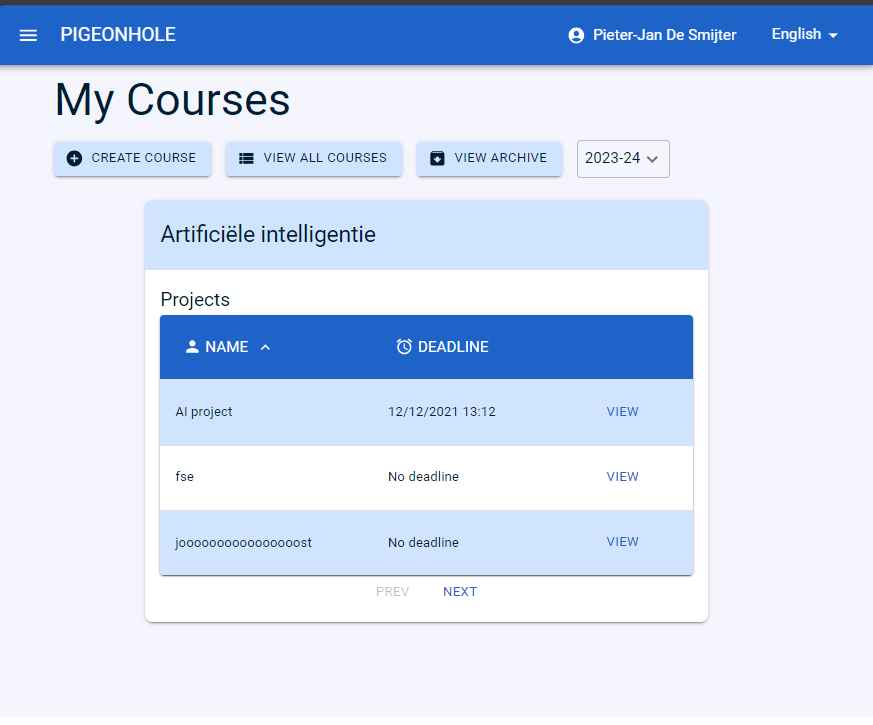
\includegraphics[width=0.75\textwidth]{images/studentpage.png}
    \caption{Home page}
\end{figure}

\subsubsection{Archived courses}
Courses of previous years are archived and can be viewed by clicking on the "Archived courses" button.

\subsubsection{Filter courses}
You can filter the courses by school year by clicking on the dropdown menu on the homepage, this will show a list of all archived courses.

\subsubsection{View deadlines}
When navigating to the calendar page from the home screen, you can see all deadlines of the projects you are enrolled in. 

\begin{figure}[H]
    \centering
    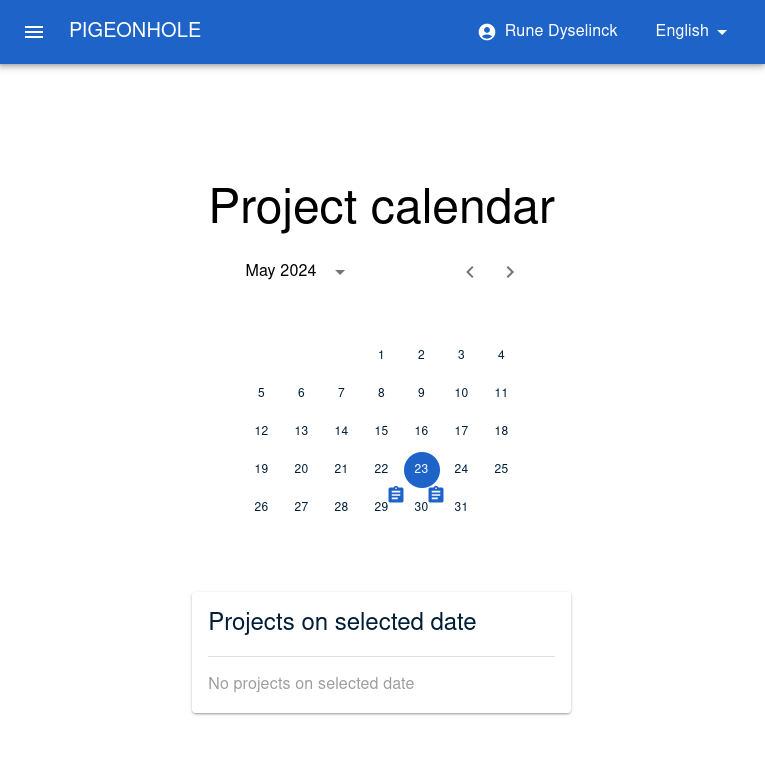
\includegraphics[width=0.75\textwidth]{images/calendar.png}
    \caption{Calendar page}
\end{figure}

\subsection{Join a new course}
There are two types of courses: public and private.
In case the course is private, you need to be invited by the teacher to join the course.


In case the course is public, you can either also be invited by the teacher or join the course yourself. 
To get a list of the public courses, click the "all open courses" button on the homepage.
On the "all open courses" page, you can see all public courses. By clicking on the "Join" button, you can join the course.

\begin{figure}[H]
    \centering
    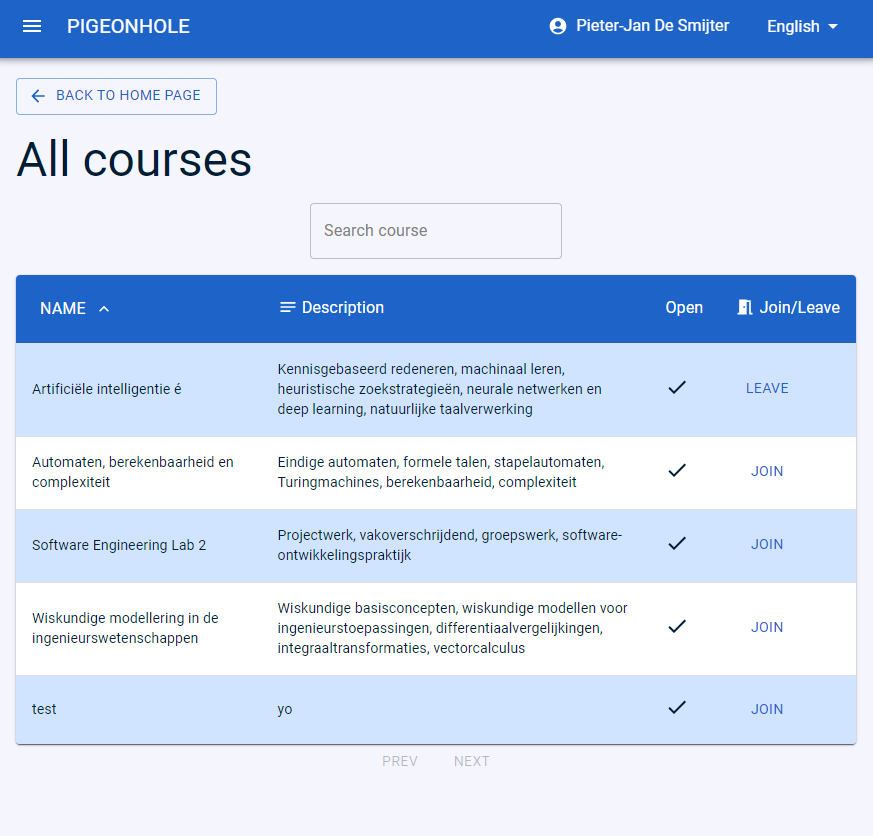
\includegraphics[width=0.75\textwidth]{images/allcourses.png}
    \caption{All open courses page}
\end{figure}

\subsection{Get an overview of the projects of a course}
On the home page, you can click on the course title to navigate to the course page. Here you can see all the projects of the course. You can see the status of the project and the deadline.
On the home page, you can also click on the "View project" button to navigate to a specific project page.
From the course page, you can also navigate to the project page by clicking on the "View project" button.


\begin{figure}[H]
    \centering
    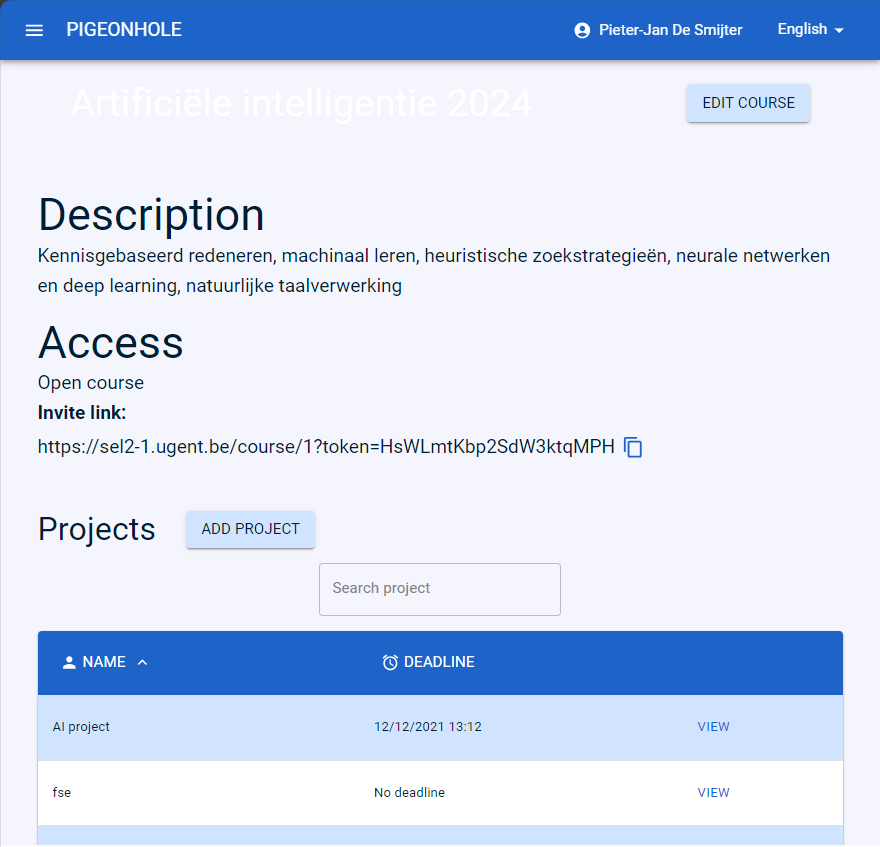
\includegraphics[width=0.75\textwidth]{images/course_page.png}
    \caption{Course page}
\end{figure}


\begin{figure}[H]
    \centering
    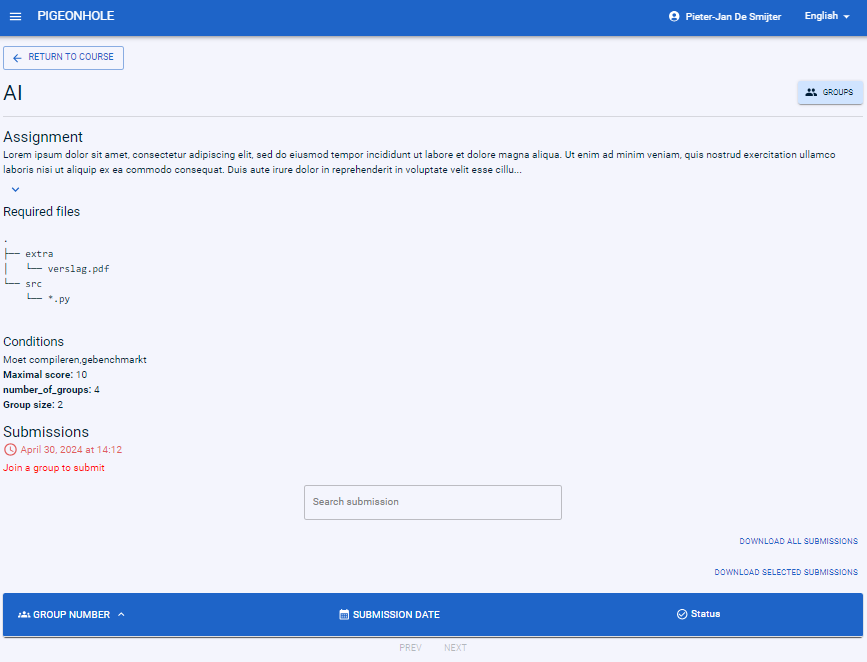
\includegraphics[width=0.75\textwidth]{images/projectpage.png}
    \caption{Project page}
\end{figure}

\subsection{Joining a group for a project}
If a project requires you to work in a group, you can view all groups by clicking on the "View groups" button on the project page. Here you can see all groups and their members. You can join a group by clicking on the "Join group" button.

\subsection{Handing in a submission}
If you want to hand in a submission, you can do this by clicking on the "Make a submission" button on the project page. On the submit page, you can upload your files and submit them by dragging them into the dropzone or by clicking on the dropzone and selecting the files.

\begin{figure}[H]
    \centering
    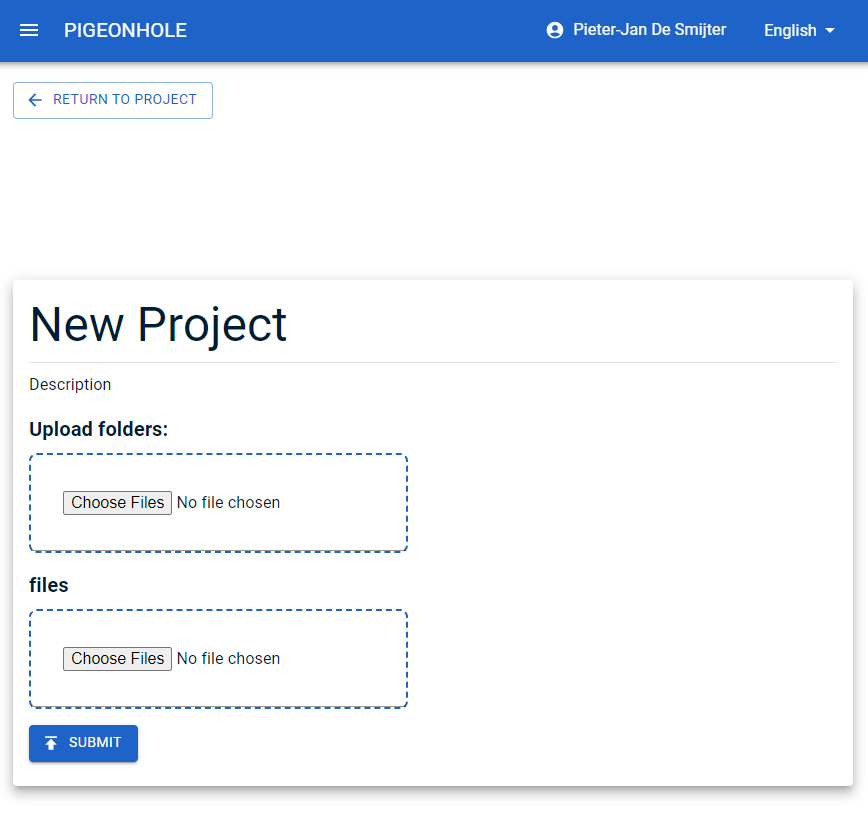
\includegraphics[width=0.75\textwidth]{images/submit.png}
    \caption{Project page}
\end{figure}

\subsection{Viewing feedback}
The automatic feedback will be immediately available after submitting and can be viewed on the submit feedback page. Here you will be able to acces the feedback of the file structure tests and advanced tests provided by the teacher.

\begin{figure}[H]
    \centering
    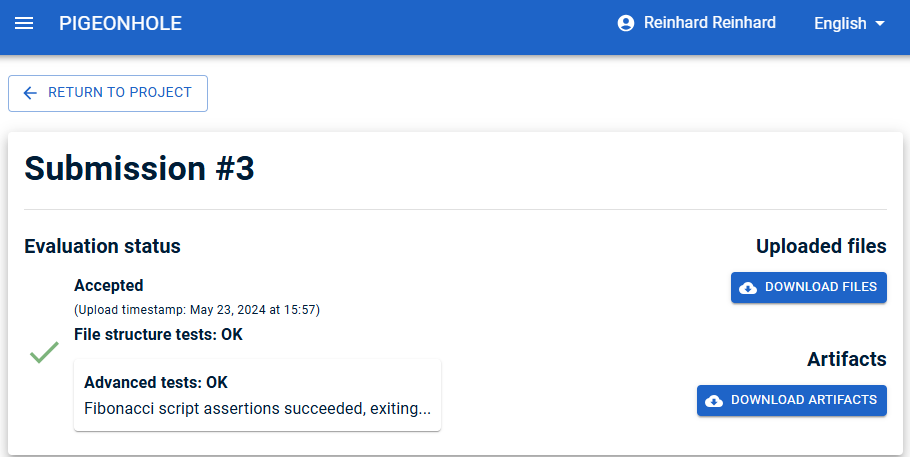
\includegraphics[width=0.75\textwidth]{images/submissionfeedback.png}
    \caption{Project page}
\end{figure}

\subsection{View your past submissions}
All your past submissions can be viewed on the project page.

\section{Teacher Section}

\subsection{Creating a Course}
Teachers can create a new course by clicking the "Create a course" button on the homepage. They can set the course name, description, and privacy settings. After creating the course, they can invite students to join with the link provided.

\begin{figure}[H]
    \centering
    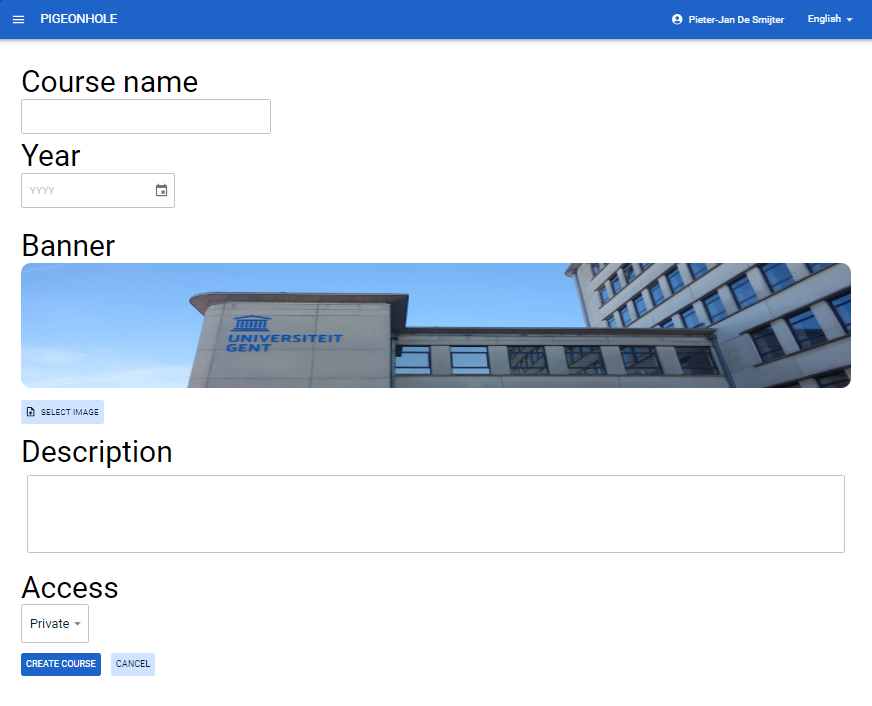
\includegraphics[width=0.75\textwidth]{images/createcourse.png}
    \caption{Create course page}
\end{figure}

\subsection{Creating a Project}
Teachers can create a new project by clicking the "Create a project" button on the course page. They can set the project name, description, and deadline. After creating the project, students can submit their work.
Teachers can also set the automatic feedback settings for the project. This ranges from directory structure to advanced test on students code. 
Here, the teacher can also set the necessary group size and amount of groups for the project.

\begin{figure}[H]
    \centering
    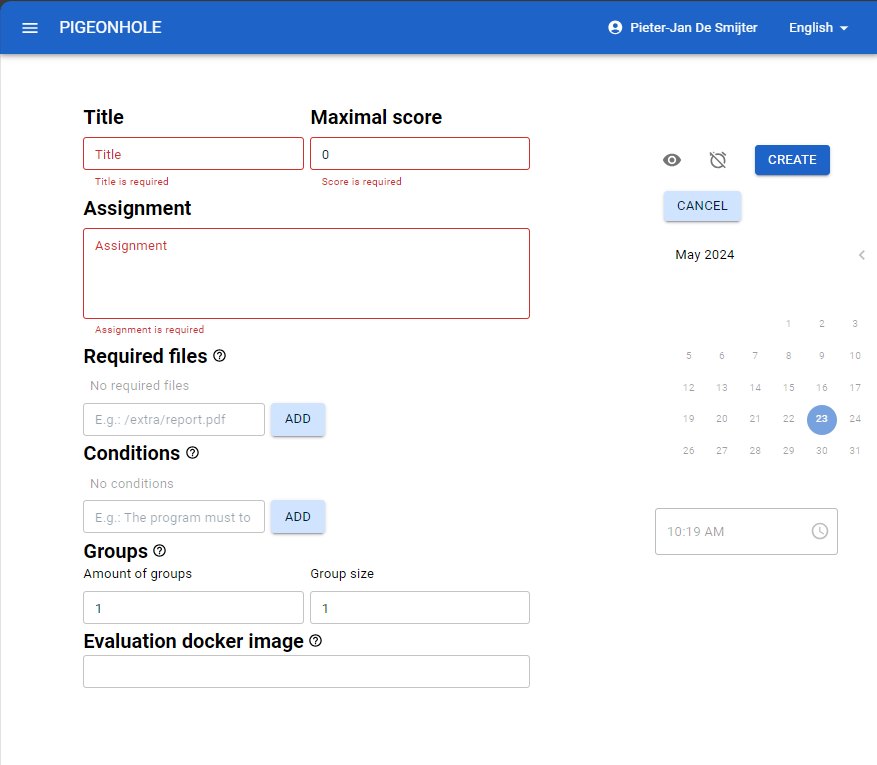
\includegraphics[width=0.75\textwidth]{images/createproject.png}
    \caption{Create project page}
\end{figure}

The teacher can also set simple and advanced tests for the project. The simple tests are run on the file structure of the submission, while the advanced tests are run on the code itself. Even when tests fail, the submission will be saved and the teacher can still view the submission.

\subsubsection{A quick quide to the simple tests}

You can add required files in the \textit{required files} field on the add/edit project page.
There are two options for adding files:

\begin{enumerate}[label=\arabic*.]
    \item \textbf{Add a specific file:} \texttt{/extra/report.pdf}\\
    In this case, the file \texttt{report.pdf} is required in the directory \texttt{extra}.
    
    \item \textbf{Add a file type:} \texttt{src/*.py}\\
    In this case, the only file type al=<lowed in the \texttt{src} directory will be Python files.
\end{enumerate}

There are also several options on how to use these files:

\begin{enumerate}[label=\arabic*.]
    \item \textbf{Required files}\\
    Using a checkmark, the files will be required and submissions without these files will be considered invalid.
    
    \item \textbf{Forbidden files}\\
    Using a crossmark, the files will be forbidden and submissions with these files will be considered invalid.
    
    \item \textbf{Maybe files}\\
    Using a question mark (?), the files will not be checked, and their presence will not affect the validity of the submission.
\end{enumerate}

\subsubsection{A quick quide to the advanced tests}

For programming projects hosted on our platform that need to verify that the code compiles/runs/gives the correct output, we offer an advanced interface to run code on each submission the moment they're submitted using docker images.

The process of setting up the advanced tests is as follows:
\begin{enumerate}[label=\textbf{\arabic*.}]
    \item \textbf{Write your tests and package them in a Docker image}
    \begin{itemize}
        \item We offer an example Docker image in \texttt{examples/advanced-evaluation}.
        \item Place the submission files in a volume under \texttt{/usr/src/submission}, output artifacts under \texttt{/usr/out/artifacts}, and determine correctness with the exit code (0 for success, other values for failure).
    \end{itemize}
    
    \item \textbf{Push your image to our private Docker registry}
    \begin{itemize}
        \item Use the command: \texttt{docker push sel2-1.ugent.be:2002/[YOUR\_IMAGE\_NAME]}
    \end{itemize}
    
    \item \textbf{Configure your project on the site}
    \begin{itemize}
        \item When creating or editing your project, fill in the Evaluation Docker image name in the text field and save.
    \end{itemize}
\end{enumerate}

You will be able to see the results and artifacts in the submission's page.

\subsection{Viewing Submissions}
Teachers can view all submissions for a project by clicking the "View submissions" button on the project page. They can see the submission status and download the files and automatic feedback.

\begin{figure}[H]
    \centering
    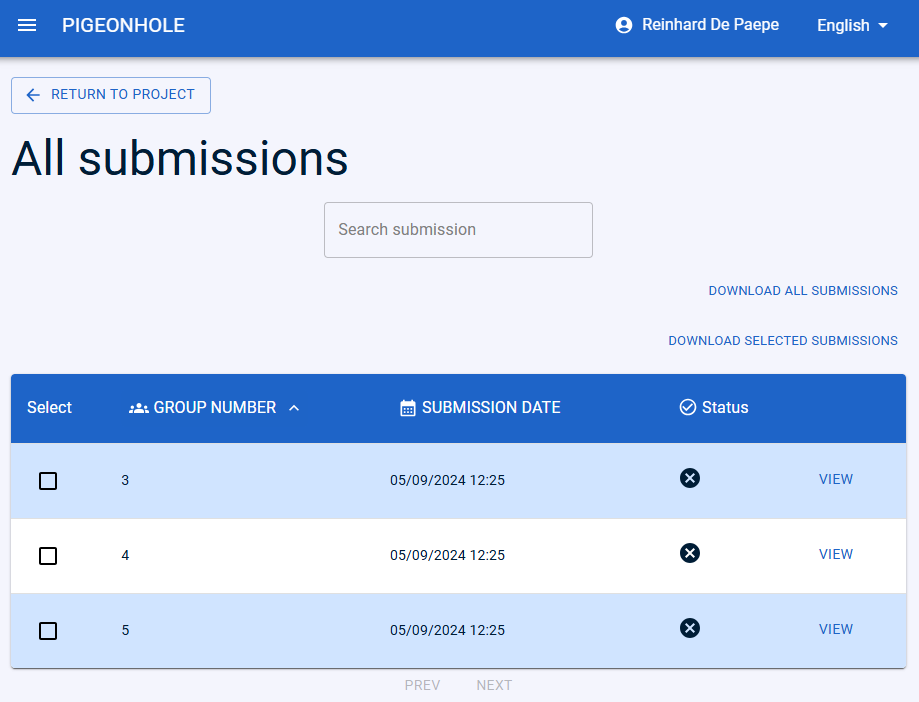
\includegraphics[width=0.75\textwidth]{images/all_submissions.png}
    \caption{All submissions page}
\end{figure}


\subsection{Viewing Courses and Projects}
Teachers can view all courses they are teaching on the homepage. By clicking on the course title, they can navigate to the course page. Here they can see all the projects of the course and the students enrolled in the course.

\subsection{Viewing students}
On the course page, teachers can see all students enrolled in the course. By clicking on the 'View students' button, they can navigate to the students' page. Here they can see all students.

\subsubsection{Removing a student from a course} 
On the view student page, teachers can select and remove students from the course.

\subsection{Adding a co-teacher}
You can use the course link to invite a co-teacher to the course. The co-teacher will have the same rights as the teacher.

\subsection{Viewing co-teachers}
Similarly to students, teachers can see all co-teachers on the course page. By clicking on the 'View co-teachers' button, they can navigate to the co-teachers' page.

\subsection{Editing a course or project}
Teachers can edit a course or project by clicking on the 'Edit' button on the course or project page. Here they can change the course or project name, description, or deadline. The edit panel looks the same as the create panel, but with the fields filled in.

\section{Admin Section}

Admins have the same functionality as teachers, but can also edit users. Admins have in the sidebar a button to navigate to the user page. Here they can see all users and edit them.

\subsection{Editing or Deleting a user}
Admins can edit a user by clicking on the 'Edit' button on the user page. Here they can change the user's name, email, or role. They might also opt to delete the user by clicking the 'Delete' button on the user page.

\section{A bit more information on the lists}
The lists of courses, projects, and submissions are paginated. You can navigate through the pages by clicking on the page number or the next/previous buttons.
Most lists are also filterable by typing in the search bar, and you can sort the list by clicking on the column headers.

\section{Troubleshooting}
If you encounter any issues while using the platform, please contact our support team for assistance. You can reach us via email at 'axel.lorreyne@ugent.be'.

\section{Conclusion}
This user manual covers the basic functionality of the PigeonHole Project Submission Platform for students, teachers, and administrators. For technical information, you can view our GitHub repository at \url{https://github.com/SELab-2/UGent-1/}.

\end{document}
